\chapter{Technische Machbarkeit}\label{ch:technische-machbarkeit}
Nachfolgend sollen die technologischen Entscheidungen für unser System erfolgen
und die technische Machbarkeit dieser Objektorientierten Analyse nachgewiesen werden.
Um die Technologien einschränken zu können, werden (Ausschluss-)Kriterien definiert,
nach welchen die verschiedenen Technologien bewertet werden.
Diese leiten sich maßgeblich aus verschiedenen Einflussfaktoren ab.
Konkret sind dabei diese fünf Faktoren zu nennen:

\begin{itemize}
    \item Entwickler/Zulieferer
    \item Unternehmen
    \item Markt
    \item Zeit
    \item Gesetze
\end{itemize}

Bei der Auswahl der Technologien wird sich auf vier Schichten bezogen,
welche den Stack für dieses System darstellen.
Diese Schichten lauten:
\begin{itemize}
    \item Hardware
    \item Betriebssystem
    \item Programmiersprache
    \item Bibliotheken
\end{itemize}
Dabei ist wichtig zu überprüfen, ob die ausgewählten Technologien
aus den verschiedenen Schichten miteinander kompatibel sind.

Auch auf die Notwendigkeit einer Alternative zur Übergabe des Ergebnisses der Plagiatsprüfung,
falls das HTTP-Timeout ausläuft, wird hierbei eingegangen.

Sobald die Technologieentscheidungen getroffen wurden,
wird die technische Machbarkeit des geplanten Systems bewiesen.
Dazu wird ein Prototyp erstellt, welcher kritische Punkte des Systems abdeckt.
Mit kritischen Punkte sind dabei solche Teile des Systems gemeint,
ohne die das gesamte System nicht funktionieren würde.
Konkret haben sich bei der Analyse drei Punkte herausgestellt,
welche kritisch für das Gesamtsystem sind:
\begin{itemize}
    \item REST Schnittstelle
    \item Auslesen der PDF
    \item Schnittstelle zu chatbasierter KI zur Plagiatsprüfung
\end{itemize}


\section{(Ausschluss-)Kriterien}\label{sec:ausschlusskriterien}

\paragraph{Freie Verwendung (Gesetze)}\label{par:freie-verwendung}
Das erste Ausschlusskriterium ist die freie Verwendung der Technologien.
Dabei ist wichtig zu betonen, dass durch Gesetze bzw.\ Lizenzen die
Verwendung der Technologie nicht eingeschränkt werden soll.

\paragraph{Weite Verbreitung (Entwickler, Unternehmen, Markt, Zeit)}\label{par:weite-verbreitung}
Eine weite Verbreitung der verwendeten Technologien muss gegeben sein.
Dies bedeutet, dass es marktüblich sein soll , diese Technologie für den
konkreten Anwendungsfall in unserem System zu verwenden.

Ableiten lässt sich dieses Kriterium aus den Faktoren Entwickler, Unternehmen, Markt und Zeit.
Die Entwickler können bei einer weit verbreiteten Technologie
auf eine große Wissensbasis zu dieser Technologie zugreifen.
Ebenso hat das auftraggebende Unternehmen den Vorteil, dass die Entwicklungskosten geringer sind,
wenn bereits bewährte Technologien benutzt werden, und nicht von neu auf etwas entwickelt werden muss.

In diesem Zusammenhang ist auch die Entwicklung der Technologie auf dem
Markt in den letzten Jahre zu beachten.
So ist es ebenfalls entscheidend, ob eine Technologie gerade im Aufschwung
ist oder das Ende des Lebenszyklus erreicht hat.
Dadurch kann eine Langlebigkeit des Systems gewährleistet werden.

\paragraph{Performance (Unternehmen, Markt)}\label{par:performance}
Die Performance des Systems ist ein wichtiger Aspekt der Technologieentscheidung.
Umso schneller unser System ein Ergebnis an den BachelorChecker weitergeben kann,
desto besser ist auch die Erfahrung des Benutzers mit der Applikation.

Auch in Bezug auf die Langlebigkeit des Systems ist die Performance ein wichtiger Faktor.
Durch eine hohe Performance kann die Lebensdauer des Systems verlängert, oder die Effizienz gesteigert werden.

\paragraph{Skalierbarkeit (Unternehmen)}\label{par:skalierbarkeit}
Auch die Skalierbarkeit der Technologien ist entscheidend.
Dabei muss beachtet werden, dass bei Wachstum des Unternehmens auch das System mitwachsen muss.
Dementsprechend muss auch der \ac{AiPC} den
Herausforderungen einer gestiegenen Nachfrage gewachsen sein.

\paragraph{Sicherheit (Gesetz, Unternehmen)}\label{par:sicherheit}
Die Sicherheit der Nutzerdaten darf durch die verwendeten Technologien nicht gefährdet werden.
Je nach Art der Bachelorarbeit kann es vorkommen, dass diese vertrauliche Informationen enthält,
die nicht an die Öffentlichkeit gelangen dürfen.
Dies ist zum einen rechtlich nicht erlaubt, zum anderen würde das auftraggebende Unternehmen
dadurch einen erheblichen Schaden, sowohl durch mögliche Klagen als auch auf das Image bezogen, erleiden.


\section{Technologieentscheidungen}\label{sec:technologieentscheidungen}
Nachfolgend werden die Technologieentscheidungen für die verschiedenen Schichten des Systems getroffen.
Dabei wird zuerst die Entscheidung für das Betriebssystem getroffen,
da dieses die Grundlage für die weiteren Entscheidungen bildet.

Die restlichen Schichten müssen dementsprechend mit dem Betriebssystem kompatibel sein.

\subsection{Betriebssystem}\label{subsec:betriebssystem}
Bei der Wahl des Betriebssystems gibt es grundsätzlich drei Möglichkeiten,
welche aufgrund der Marktsituation in Betracht gezogen werden können.
So sind Windows, MacOS und Linux die drei meistverbreiteten Betriebssysteme für die Entwicklung von Software\autocite{JetBrains-2023}.

Da es sich bei Linux als einzige der drei Optionen um ein Open-Source Betriebssystem handelt,
ist dieses für die Verwendung in diesem System am besten geeignet.
So profitiert Linux von der großen Entwicklergemeinde, welche das Betriebssystem stetig weiterentwickelt.
Auch die Sicherheit ist bei Linux im Vergleich zu den anderen beiden Betriebssystemen am höchsten,
da es sich um ein Open-Source Betriebssystem handelt und somit jeder die Möglichkeit hat,
den Quellcode einzusehen und mögliche Sicherheitslücken zu finden und zu beheben.

Unter den verschiedenen Linux Distributionen gibt es viele Möglichkeiten, welche für die Verwendung in diesem System geeignet sind.
Dabei ist es wichtig, dass die Distribution eine lange Unterstützungsdauer hat.
Unsere Empfehlung ist hierbei Ubuntu Server, da diese Distribution eine Unterstützungsdauer bis 2032 garantiert\autocite{ubuntu}.

\subsection{Hardware}\label{subsec:hardware}
Bei der Auswahl der Hardware ist es wichtig, dass diese mit dem ausgewählten Betriebssystem kompatibel ist.
Laut eigener Aussage ist Ubuntu Server mit allen gängigen Prozessorarchitekturen kompatibel\autocite{ubuntu}.

Dazu gehören unter anderem x86-64, ARM v7 und ARM64, welche zu den meistverbreiteten Prozessorarchitekturen gehören.
Die letztendliche Auswahl der Hardware kann an diesem Punkt allerdings noch nicht getroffen werden,
da die Hardwareanforderungen des Systems noch nicht bekannt sind.
Auch die bereits vorhandene Hardware des auftraggebenden Unternehmens spielt hierbei eine Rolle.

Sobald die Hardwareanforderungen des Systems bekannt sind, kann die Auswahl der Hardware getroffen werden.

\subsection{Programmiersprache}\label{subsec:programmiersprache}
Ein weiterer wichtiger Aspekt bei der Umsetzung des Systems ist die Programmiersprache.
Zusätzlich zu den bereits genannten Ausschlusskriterien kommen hierbei noch weitere Kriterien hinzu,
die sicherstellen sollen, dass die Sprache optimal für den konkreten Anwendungsfall verwendet werden kann.
Diese Kriterien sind eingeteilt in “Muss”- und “Kann”-Kriterien.
Folgende Kriterien müssen erfüllt werden:
\begin{itemize}
    \item \textbf{Objektorientierung} Die Sprache muss es ermöglichen, objektorientiert zu programmieren
    \item \textbf{REST-fähig} Die Sprache muss es ermöglichen, dem Kundensystem BachelorChecker eine REST-Schnittstelle bereitzustellen
    \item \textbf{Testfähigkeit} Die Sprache muss es ermöglichen, das System systematisch ohne großen Mehraufwand zu testen
\end{itemize}

Nachfolgende Kriterien hingegen sind optional, fließen aber
positiv in den Entscheidungsprozess ein, falls diese erfüllt werden:
\begin{itemize}
    \item \textbf{Entwicklungsfähigkeit im Bereich KI} Die Sprache sollte es ermöglichen, eine KI zu entwickeln.
    Dies ist insbesondere für mögliche Weiterentwicklungen des Systems hilfreich,
    bei denen beispielsweise die KI zur Plagiatsprüfung selbst entwickelt werden soll.
    \item \textbf{Generierung von Dokumentation} Die Sprache sollte es ermöglichen, Dokumentation für den Code
    automatisch generieren zu lassen, um den manuellen Dokumentationsaufwand gering zu halten.
\end{itemize}
Unter dem Aspekt der weiten Verbreitung der Programmiersprachen
stechen vornehmlich die Sprachen Java, Python und JavaScript hervor.
Laut einer Statistik von Statista sind dies weltweit die drei beliebtesten Programmiersprachen\autocite{programmiersprachen}.
Somit ist der Aspekt der weiten Verbreitung bei allen gegeben.
Auch der Aspekt der Kompatibilität mit den darunterliegenden Systemschichten ist gegeben.
Die weiteren Kriterien zur Technologieentscheidung werden nachfolgend überprüft.

\begin{table}[H]
    \begin{tabularx}{\textwidth}{l|X|X|X}
        ~                                      & \textbf{Java}                                                            & \textbf{Python}                                                                  & \textbf{JavaScript}                                                     \\ \hline
        \textbf{Freie Verwendung}              & \cellcolor{red!30} Proprietär                                            & \cellcolor{green!30}Ja                                                           & \cellcolor{green!30}Ja                                                  \\ \hline
        \textbf{Skalierbarkeit}                & \cellcolor{green!30}Hoch                                                 & \cellcolor{orange!30}Mittel                                                      & \cellcolor{green!30}Am Höchsten                                         \\ \hline
        \textbf{Performance}                   & \cellcolor{green!30}Hoch                                                 & \cellcolor{green!30}Hoch                                                         & \cellcolor{red!30}Niedrig                                               \\ \hline
        \textbf{Objektorientierung}            & \cellcolor{green!30}Ja                                                   & \cellcolor{green!30}Ja                                                           & \cellcolor{green!30}Ja                                                  \\ \hline
        \textbf{REST-fähig}                    & \cellcolor{green!30}Ja, z.B.\ mit Spring                                 & \cellcolor{green!30}Ja, z.B.\ mit Flask & \cellcolor{green!30}Ja, z.B.\ mit node.js \\ \hline
        \textbf{Testfähig}                     & \cellcolor{green!30}Ja                                                   & \cellcolor{green!30}Ja                                                           & \cellcolor{green!30}Ja                                                  \\ \hline
        \textbf{Entwicklung einer KI}          & \cellcolor{orange!30}Ungewöhnlich, aber möglich mit z.B.\ Deeplearning4j & \cellcolor{green!30}Beliebteste Programmiersprache im Kontext von KI-Entwicklung & \cellcolor{orange!30}Ungewöhnlich, aber möglich mit z.B.\ TensorFlow.js \\ \hline
        \textbf{Generierung der Dokumentation} & \cellcolor{green!30}Möglich mit z.B.\ JavaDoc & \cellcolor{green!30}Möglich mit z.B.\ Doxygen & \cellcolor{green!30}Möglich mit z.B.\ JSDoc \\
    \end{tabularx}
    \caption{Technologieentscheidung Programmiersprache}
    \label{tab:technologieentscheidung-programmiersprache}
\end{table}
Die Punkte Freie Verwendung, Skalierbarkeit und Performance beziehen sich auf nachfolgende Quelle\autocite{nodejavapython}.

Aus der abgebildeten Tabelle geht hervor, dass es sich bei Java um eine proprietäre Programmiersprache handelt.
Somit ist der Aspekt der freien Verwendung nicht gegeben und Java scheidet für die Verwendung dieses Systems aus.

Die Programmiersprachen Python und JavaScript erfüllen beide grundsätzlich die genannten Kriterien.
Auch der Punkt Performance ist bei beiden Sprachen gegeben, da bei diesem System
vor allem die chatbasierte KI die Performance des gesamten Systems beeinflusst.
Aus langjähriger Erfahrung der Entwickler ist bekannt, dass die
Performance von Python und JavaScript für die Entwicklung des Systems ausreichend ist,
auch wenn Python in der Regel als etwas performanter gilt.
Somit sind beide Sprachen grundsätzlich für die Entwicklung des Systems geeignet.
Ausschlaggebend für die Entscheidung ist der Punkt der Entwicklungsfähigkeit einer KI.
Da in zukünftigen Weiterentwicklungen des Systems auch die Option bestehen soll, eine KI zur Plagiatsprüfung selbst zu entwickeln,
ist es wichtig, dass die Programmiersprache dies auch ermöglicht.
Dementsprechend ist Python in diesem Anwendungsfall die bessere Wahl, da diese Programmiersprache
die meistverwendete Programmiersprache für die Entwicklung von Künstlicher Intelligenz ist.

\subsection{Bibliotheken}\label{subsec:bibliotheken}
Der letzte Schritt bei der Auswahl der Technologien ist die Auswahl der Bibliotheken.
Dabei ist es wichtig nur Bibliotheken zu verwenden, welche auch mit der zuvor ausgewählten Programmiersprache kompatibel sind.

Weitergehend liegt bei der Auswahl der Bibliotheken der Fokus auf den kritischen
Punkten des Systems, welche bereits am Anfang des Kapitels genannt wurden.

\subsubsection{REST}\label{subsubsec:rest}
Der erste kritische Punkt des Systems ist die REST-Schnittstelle zum Kundensystem.
Laut einer Umfrage von Stack Overflow sind Django und Flask in diesem Kontext die beliebtesten
Bibliotheken, um in Python Web Anwendungen umzusetzen\autocite{webframeworks}.
Somit ist der Punkt der weiten Verbreitung bereits gegeben.

In einer gegenüberstellung der beiden Frameworks ergibt sich, dass Flask eine einfachere
Benutzung und mehr Flexibilität auszeichnet\autocite{flaskdjango}.
Da Flexibilität und Skalierbarkeit wichtige Punkte in der Umsetzung des Systems darstellen,
wurde sich letztendlich für Flask entschieden.
Auch die schnelle Lernkurve hat dabei eine Rolle gespielt.
So kann einfacher die Machbarkeit anhand eines Prototyps bewiesen werden.

\subsubsection{Auslesen der PDF}\label{subsubsec:pdf}
Der nächste kritische Punkt des Systemablaufs ist das Auslesen der PDF-Dateien.
Hierzu soll eine Bibliothek verwendet werden, welche diese Funktionalitäten bereitstellen kann.
Dabei wird die Annahme gemacht, dass die PDF-Dateien in einem maschinenlesbaren Format vom BachelorChecker bereitgestellt werden.

Die Auswahl an Bibliotheken ist hierbei sehr umfassend.
Die Wahl fiel letztendlich auf die Bibliothek pypdf.
Diese Bibliothek ist einfach zu verstehen und erhält regelmäßig Updates.
Somit ist auch hier die Langlebigkeit des Systems gewährleistet.

\subsubsection{Schnittstelle zu chatbasierter KI}\label{subsubsec:ki}
Der letzte kritische Punkt des Systems ist die Schnittstelle zu der chatbasierten KI.
Hierbei ist es wichtig, dass die Bibliothek die Möglichkeit bietet, die KI über eine Schnittstelle anzusprechen.
Da die KI in Python entwickelt werden soll, ist es wichtig, dass die Bibliothek auch mit Python kompatibel ist.

\paragraph{Das LargeLanguageModel (chatbasierte KI)} auszuwählen ist nicht einfach,
da es eine Vielzahl verschiedener Modelle und Anbieter gibt.
Für die kommerzielle Nutzung ist es wichtig, dass das Modell auch kommerziell genutzt werden darf.
Auch wie verbreitet das Modell ist, muss berücksichtigt werden.
Die Auswahl beschränkt sich somit auf folgende Modelle

\begin{table}[H]
    \begin{tabularx}{\textwidth}{lll}
        \toprule
        \textbf{LM}  & \textbf{Initial Release} & \textbf{Developer} \\
        \midrule
        Bard         & 2023-03-21               & Google             \\
        ChatGPT      & 2022-11-30               & OpenAI             \\
        Claude       & 2023-03-14               & Anthropic          \\
        Cohere       & 2021-11-15               & Cohere             \\
        Jurassic     & 2021-08-11               & AI21               \\
        Inflection-1 & 2023-06-22               & Inflection AI      \\
        \bottomrule
    \end{tabularx}
    \caption{Kommerzielle LLMs}\autocite{sapling.llmindex}
    \label{tab:kommerzielle-llms}
\end{table}



Unter den betrachteten Modellen wird ChatGPT mit GPT-3 für die technische Machbarkeit und den Prototyp ausgewählt.
Die Entscheidung für dieses Modell basiert auf der Vergabe von OpenAI-API-Keys, was eine kostengünstige und wenig aufwändige Nutzung ermöglicht.
Zudem zeichnet sich ChatGPT durch seine weite Verbreitung aus, wie aus aktuellen Statistiken hervorgeht~\autocite{statista.gpt}.

ChatGPT ist eine Ableitung des Large Language Models (LLM) GPT-3 von OpenAI, welches 175 Milliarden Parameter umfasst~\autocite[][S. 5]{openai.gpt}.
Damit ist es das umfangreichste Modell unter den genannten Alternativen~\autocite{statista.gpt}.
Die Trainingsdaten für dieses Modell belaufen sich auf 45 Terabyte komprimierten Texts, was es zu einem der intensivsten und am besten trainierten Modelle in dieser Auswahl macht~\autocite[][S. 8]{openai.gpt}.
Obwohl GPT-3 im Vergleich zu anderen Modellen eine gewisse Geschwindigkeitseinbuße aufweist, zeichnet es sich durch qualitativ bessere Ergebnisse aus~\autocite{mindsdb.llm}.
Jedoch sind die Antwortzeiten von GPT-3 so marginal, dass diese kein Problem für die Nutzung in diesem System darstellen.
Diese liegen bei der Generierung von 512 Token etwa zwischen 10 und 15 Sekunden~\autocite{gptforwork.gpt3}.
Durch intensives Testen konnte ebenfalls festgestellt werden, dass die Antwortzeiten schnell genug sind, um nicht in einen HTTP-Timeout zu laufen.

Für einen produktiven Einsatz empfiehlt der Auftragnehmer GPT-4 Turbo zu verwenden.
Dieses Modell zeichnet sich durch eine erhöhte Verarbeitungsgeschwindigkeit und eine gesteigerte Ergebnisqualität aus.
Darüber hinaus unterstützt es eine größere Anzahl an Token~\autocite{openai.gpt4}, dadurch können auch umfangreichere Texte verarbeitet werden.
Diese Eigenschaft erweist sich als besonders vorteilhaft bei der Verarbeitung von Bachelorarbeiten.
Die Anzahl der maximalen Token beträgt 128.000~\autocite{openai.gpt4}.
Das entspricht über 300 Seiten Text~\autocite{openai.blog.gpt4}.
Ein weiterer Vorteil von GPT-4 liegt in seinem Training mit aktualisierten und umfangreicheren Datensätzen.
Dies trägt dazu bei, die Qualität der erzeugten Ergebnisse weiter zu steigern.
Außerdem bietet dieses Modell einen \ac{JSON}-Mode, welcher die Benutzung von \ac{JSON}-Strukturen erleichtert~\autocite{openai.gpt4}.
Die Antwortzeiten betragen bei GPT-4 Turbo 8-16 Sekunden~\autocite{nuvalence.gpt4}.
Dabei ist die Antwortzeit unabhängig von der Größe des übergebenen Textes~\autocite{nuvalence.gpt4}.
In Verbindung mit dem KI-System besteht für das Gesamtsystem somit keine Gefahr,in ein HTTP-Timeout zu laufen

Für die Interaktion mit dem Modell kommt das \texttt{openai package} zum Einsatz.
Diese Entscheidung basiert auf der Benutzerfreundlichkeit des Pakets sowie auf der Gewissheit,
dass es kontinuierlich von OpenAI selbst weiterentwickelt wird und somit stets auf dem aktuellen Stand ist.

% TODO Argumentation, dass wir in keine Timeouts laufen --> deswegen keine Alternative in ursprünglicher OOA

\subsection{Alternative zur Übergabe der Antwort}\label{subsec:alternative-zur-uebergabe-der-antwort}
Wie aus dem vorherigen Abschnitt hervorgeht, ist für unser System eine Alternative zur Übergabe der Antwort
an den BachelorChecker nicht notwendig.
Sollte das auftraggebende Unternehmen allerdings in Zukunft ein anderes KI-System verwenden wollen (z.B.\ ein selbst entwickeltes System),
dann kann es auch passieren, dass die Antwort nicht innerhalb des HTTP-Timeouts zurückgegeben werden kann.

In diesem Fall sollte eine Alternative zur Übergabe der Antwort an den BachelorChecker implementiert werden.
Vorbereitend auf diesen Fall soll nachfolgend eine mögliche Alternative vorgestellt werden.
Dabei wird auch darauf eingegangen, wie diese Alternative in das System integriert werden kann.

Hierbei ist es üblich, nach dem Timeout den Statuscode 202 zurückzugeben.
Dieser bedeutet, dass die Anfrage akzeptiert wurde, aber noch nicht bearbeitet werden konnte\autocite{mozilla}.
Bei dieser Antwort wird dem BachelorChecker die ID inklusive der Webadresse des Auftrags mitgegeben,
welche dieser dann in regelmäßigen Abständen abfragen kann, um den aktuellen Status des Auftrags zu erhalten.

Sollte der Auftrag in der Zwischenzeit fertig werden, dann wird auf diese regelmäßigen Abfragen das Ergebnis
der Plagiatsprüfung weitergegeben.

Eine Integration dieser Funktion in den \ac{AiPC} könnte wie folgt aussehen:
\begin{figure}[H]
    \centering
    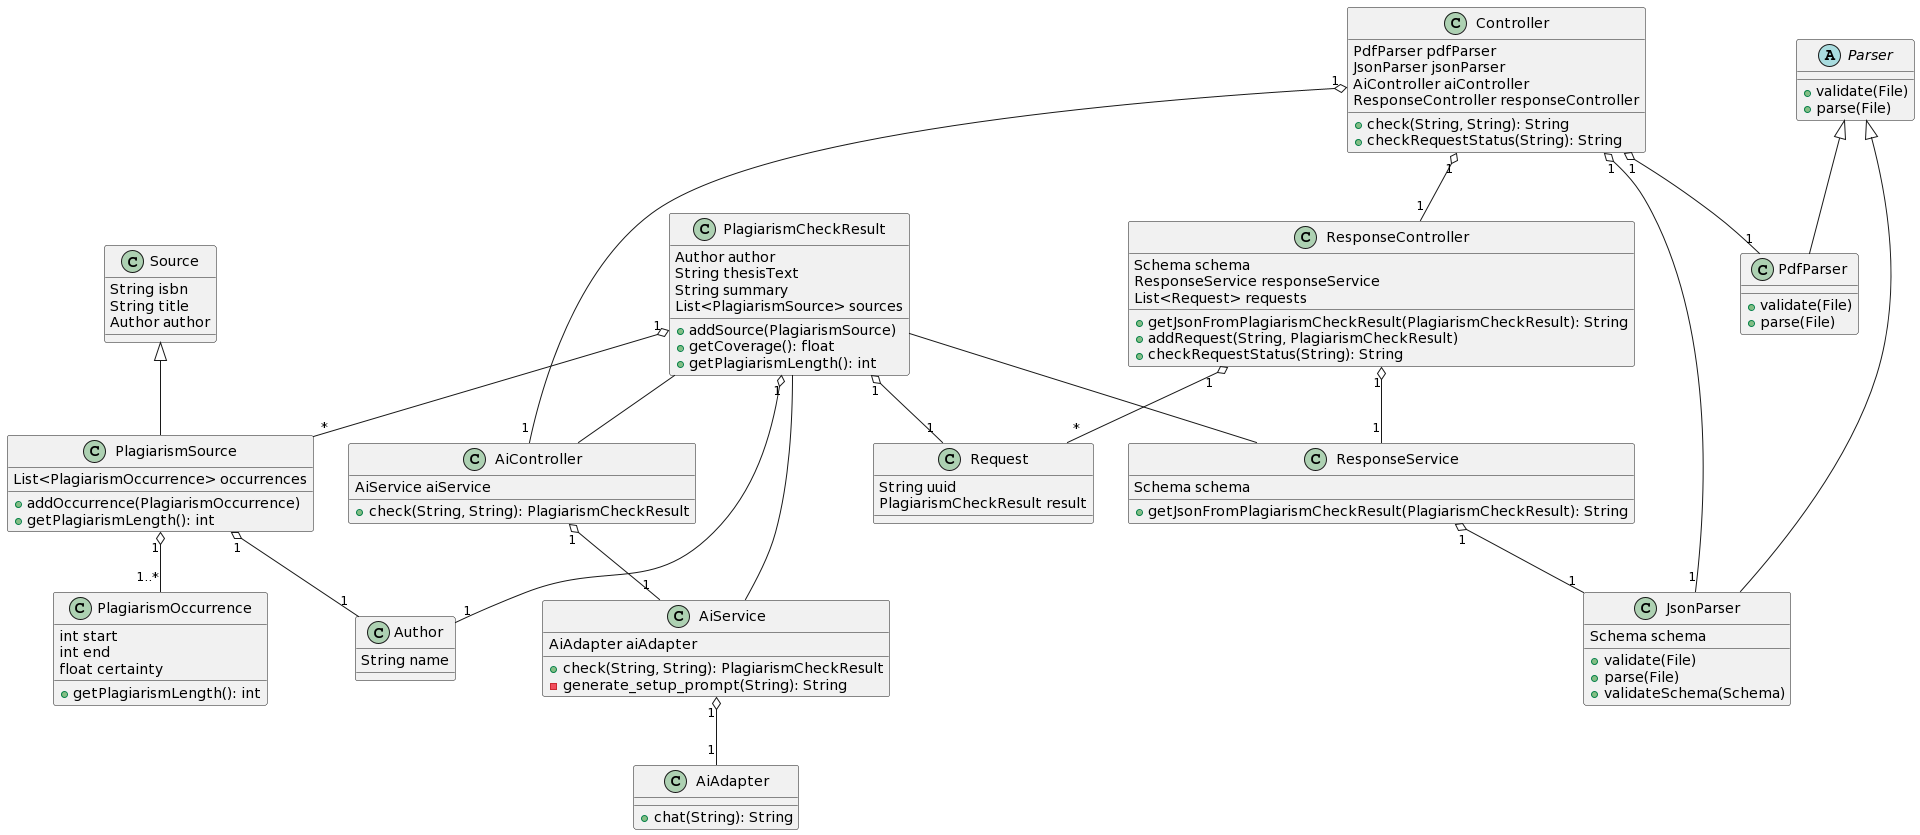
\includegraphics[width=\textwidth]{images/diagrams/Klassendiagramm_HTTP_202}
    \caption{Klassendiagramm mit Timeout-Handling}
    \label{fig:klassendiagramm-mit-timeout-handling}
\end{figure}

Die Anfragen an den \ac{AiPC} werden hierbei nach wie vor über den selben Endpunkt gestellt.
Allerdings erhält der BachelorChecker hierbei sofort eine Antwort mit dem \ac{HTTP}-Statuscode 202 und einer \ac{URL}.
Mithilfe dieser \ac{URL} kann der BachelorChecker in regelmäßigen Abständen den Status der Anfrage abfragen.
Hierzu wird ein zweiter Endpunkt in dem \ac{AiPC} hinzugefügt.
Intern wird je eine Anfrage durch eine Instanz der neu hinzugefügten Request-Klasse repräsentiert.
Dabei wird jede Instanz eindeutig durch eine, während der Plagiatsprüfungsanfrage generierten, \ac{UUID} identifiziert.
Diese \ac{UUID} dient außerdem der Verwaltung der einzelnen Instanzen durch den ResponseController.


\section{Machbarkeitsbeweis}\label{sec:machbarkeitsbeweis}

Nachfolgend soll die technische Machbarkeit des Systems mit den ausgewählten Technologien bewiesen werden.
Dabei werden die Geschäftsfälle aus dem Kapitel~\ref{ch:geschaftsfaelle} auf die Machbarkeit überprüft.
Sollten alle Geschäftsfälle umsetzbar sein, dann ist auch das gesamte System machbar.

Um dies zu beweisen, wird ein Prototyp erstellt, welcher diese Geschäftsfälle abdeckt.
% TODO Prototyp in Anhang einfügen und hier referenzieren

Strukturiert ist dieser Machbarkeitsbeweis nach den kritischen Punkten des Systems,
welche bereits in Kapitel~\ref{ch:technische-machbarkeit} genannt wurden.

\subsection{REST Schnittstelle}\label{subsec:rest-schnittstelle}
Um die Geschäftsfälle ``Eingang der Daten vom BachelorChecker'' (\ref{tab:eingang-der-daten-vom-bachelorchecker})
und ``Übergabe des Ergebnisses an den BachelorChecker'' (\ref{tab:ubergabe-des-ergebnisses-an-den-bachelorchecker})
auf Machbarkeit zu überprüfen, enthält der Prototyp eine REST-Schnittstelle mit flask.

In diesem Prototypen wird ein HTTP-Endpunkt unter der Wurzeladresse ``/'' bereitgestellt.
Dieser Endpunkt nimmt eine HTTP-POST Anfrage entgegen und gibt eine Antwort an den Client zurück.

Wenn dieser Endpunkt aufgerufen wird, dann werden die mitgegebenen PDF- und JSON-Dateien verarbeitet
und letztendlich eine JSON-Datei mit dem Ergebnis der Plagiatsprüfung zurückgegeben.

Somit sind die beiden genannten Geschäftsfälle mit der ausgewählten Technologie machbar.

\subsection{Auslesen der Dateien}\label{subsec:auslesen-der-dateien}
Der nächste Geschäftsfall ist das ``Auslesen der Bachelorarbeit und der Zusatzinformationen'' (\ref{tab:auslesen-der-bachelorarbeit-und-zusatzinformationen}).
Wie in der Technologieentscheidung beschrieben, wird für das Auslesen der PDF-Datei die Bibliothek pypdf verwendet.

Diese Funktionalität wurde wie folgt in den Prototypen integriert:
\begin{lstlisting}[caption={Auslesen von PDF-Dateien},captionpos=b,label={lst:pypdf}, language=Python, breaklines=true]
def parse(self, path: str) -> str:
    """
    Parse the text content of a PDF file.

    :param path: The file path of the PDF file to parse.
    :return: The parsed text content of the PDF file.
    """
    self.validate(path)
    with open(path, 'rb') as file:
        reader = pypdf.PdfReader(file)
        text = ''
        for _, page in enumerate(reader.pages):
            text += page.extract_text()
    return text
\end{lstlisting}

Ebenso wird die JSON-Datei mit den Zusatzinformationen ausgelesen.
Hierbei wird das Schema der Datei validiert.
Dieses Schema ist in Kapitel~\ref{ch:schnittstellen} beschrieben.

Zusammenfassend lässt sich somit festhalten, dass auch dieser Geschäftsfall mit den ausgewählten Technologien machbar ist.

\subsection{Schnittstelle zu chatbasierter KI}\label{subsec:schnittstelle-zu-chatbasierter-ki}
Diese ausgelesenen Daten werden anschließend aufbereitet und ein Prompt für die chatbasierte KI wird erstellt.
Dies erfüllt den Geschäftsfall ``Aufbereiten der Daten und Generierung eines Prompts für die KI'' (\ref{tab:aufbereiten-der-daten-und-generierung-eines-prompts-fur-die-ki}).

Die Erstellung des Prompts erfolgt mit einer Methode, welche die Daten in ein String-Format umwandelt,
welches von der KI verarbeitet werden kann.
\begin{lstlisting}[caption={Erstellung eines Prompts für die KI},captionpos=b,label={lst:prompt-erstellen}, language=Python, breaklines=true]
def generate_setup_prompt(self, data) -> str:
    """
    Generates a setup prompt for the AI adapter based on the given data.
    """
    return (
        f"Analyze the text for plagiarism. Author: {data['author']},"
        f"Title: {data['title']}, Language code: {data['language']}."
        f"Exclude sources with ISBNs: {data['sources']}."
        f"The response should adhere to the following JSON schema: {self.schema}"
        "Make sure all the keys have the correct value,"
        "and guarantee that the required keys are always present."
    )
\end{lstlisting}

Dieser Prompt wird zusammen mit dem Text der Bachelorarbeit im Rahmen des nächsten Geschäftsfalls
``Weitergabe der Daten an KI'' (\ref{tab:weitergabe-der-daten-an-ki}) an die KI übergeben.
Um dies umzusetzen wird die Klasse ``AIAdapter'' verwendet.
Diese Klasse enthält eine Methode ``chat'', welche die Daten an die KI übermittelt und das Ergebnis zurückgibt.
Die Implementierung ist nachfolgend zu sehen.
\begin{lstlisting}[caption={Weitergabe der Daten an KI},captionpos=b,label={lst:weitergabe-an-ki}, language=Python, breaklines=true]
def chat(self, messages: list[dict]):
    """
    Sends a list of messages to the OpenAI API and returns the response.

    Args:
    messages (list[dict]): A list of dictionaries each representing a message.

    Returns:
    json_data (dict): A dictionary containing the response from the OpenAI API.
    """
    completion = self.client.chat.completions.create(
        model="gpt-3.5-turbo-1106",
        response_format={"type": "json_object"},
        messages=messages,
    )
    json_content = completion.choices[0].message.content
    json_data = json.loads(json_content)
    return json_data
\end{lstlisting}

Dabei wird auch spezifiziert, in welchem Format die Antwort der KI zurückgegeben werden soll.
In diesem Fall wird das Format ``json\_object'' verwendet, um die Antwort möglichst einfach verarbeiten zu können.

Dieser Ausschnitt des Prototypen zeigt auch, wie die Antwort der KI erhalten wird.
Zusätzlich dazu wird das Schema dieser Antwort noch validiert und ein ``PlagiarismCheckResult''
Objekt zur internen Datenhaltung des Ergebnisses erstellt.
Somit ist auch der Geschäftsfall ``Erhalt des Ergebnisses der KI'' (\ref{tab:erhalt-des-ergebnisses-der-ki}) durch den Prototypen abgedeckt.

Zuletzt folgt noch der Geschäftsfall ``Weiterverarbeitung des Ergebnisses der KI'' (\ref{tab:weiterverarbeitung-des-ergebnisses-der-ki}).
Hierbei wird aus dem internen ``PlagiarismCheckResult'' Objekt eine JSON-Datei erstellt.
Dies erfolgt in der Klasse ``ResponseService'' mit der Methode:

\texttt{get\_json\_from\_plagiarism\_check\_result(self, data: PlagiarismCheckResult)}.

Diese Methode bringt das Ergebnis in das Format, welches in Kapitel~\ref{ch:schnittstellen} beschrieben ist.
Durch die Umsetzung im Prototypen ist somit bewiesen, dass die zuvor genannten Geschäftsfälle machbar sind.